\documentclass{report}
\usepackage[utf8x]{inputenc}
\usepackage[T1]{fontenc}
\usepackage[francais]{babel}
\usepackage{graphicx}
\usepackage{hyperref}
\author{Léo Unbekandt - Guillaume Paran - Lucas Saurel}
\date{Mai 2012}
\title{Projet web - UnsapaIPW}

\begin{document}

  \maketitle
  \tableofcontents

  \section*{Introduction}
  \addcontentsline{toc}{section}{Introduction}

  \section{Interprétation du sujet}
  \section{Organisation de l'équipe}
  \section{Schéma de données}
    Le sujet nous imposait d'utiliser un certain nombre
    auxquels nous avons ajouté un certain nombre d'attributs.

    \begin{figure}
      \caption{Schéma relationnel}
      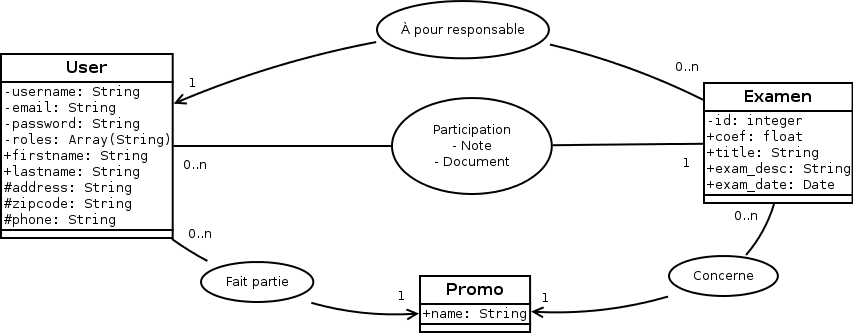
\includegraphics[width=0.9\textwidth]{./data.png}
    \end{figure}

    \begin{figure}
      \caption{Modèle physique de base de données}
      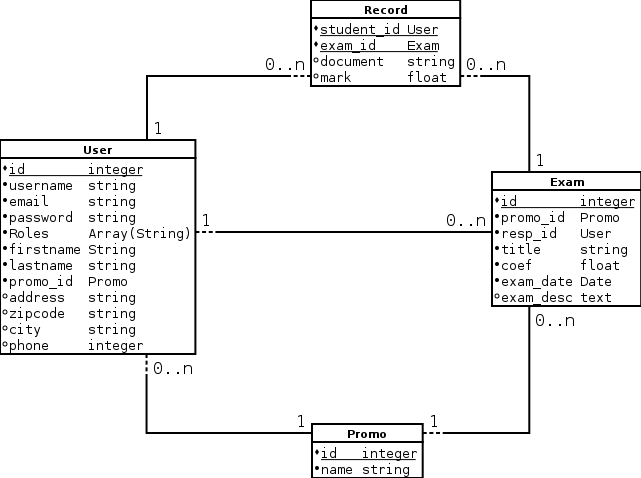
\includegraphics[width=0.9\textwidth]{./db.png}
    \end{figure}

    \subsection{User}
      En plus des champs prérequis :
      \begin{itemize}
        \item{Prénom}
        \item{Nom}
        \item{Adresse}
        \item{Code postal}
        \item{Ville}
        \item{Adresse e-mail}
        \item{Numéro de téléphone}
      \end{itemize}

      Le UserBundle nous rajoute toute la partie nécessaire à la gestion de
      l'utilisateur côté serveur.
      \begin{itemize}
        \item{Le mot de passe $\Rightarrow$ chiffré en sha1 dans la BDD}
        \item{Les rôles $\Rightarrow$ Pour la gestion des permissions}
        \item{Nom d'utilisateur}
        \item{Expiration du compte, confirmation par email etc.}
      \end{itemize}

      Et enfin nous avons ajouté un champs pour notre besoin qui est une
      promotion, en effet, on considère qu'un étudiant appartient à une
      promotion précise.

    \subsection{Promo}
      Les promotions correspondent à un regroupement d'utilisateur, dans le
      cas d'utilisation présent, tous les étudiants d'une même année 
      appartiennent à une promotion unique.

    \subsection{Exam}
      
    \subsection{Record}


  \section{Réalisation Technique}
    \subsection{UserBundle}
      Nous avons utilisé un Bundle d'extension nommé : 
      \href{https://github.com/FriendsOfSymfony/FOSUserBundle}{UserBundle}.
      
      Ce bundle constitue la brique applicative qui permet d'effectuer toutes
      les actions nécessaire à presque tous les projets, c'est-à-dire :
      \begin{itemize}
        \item{Inscription}
        \item{Authentification}
        \item{Connexion}
        \item{Déconnexion}
        \item{Gestion du profil}
        \item{Changement de mot de passe}
      \end{itemize}
      Nous évitant du travail laborieux qui ne sert pas sur le plan métier de
      l'application.

    \subsection{Les tests avec PHPUnit}
    \subsection{La documentation développeur avec phpDocumentor}

  \section*{Conclusion}
  \addcontentsline{toc}{section}{Conclusion}

\end{document}
